\section{Arquitectura Kappa}

\subsection{Descripción General}

La Arquitectura Kappa surge en 2014 como respuesta de parte de Jay Kreps a la Arquitectura Lambda. 
Si bien Lambda puede describirse de forma "sencilla" como una serie de transformaciones y además pone 
mucho enfasis en la posibilidad y facilidad de reprocesar los datos; 
tiene la desventaja de obligar a mantener código que debe producir el mismo resultado en dos sistemas
distribuidos. Esto implica que cualquier cambio o mejora que reciba uno debe recibir un tratamiento
de reingenieria para que el otro también lo tenga. Y, según argumenta Jay Kreps, la tendencia es a 
optimizar el código para uno de los motores (incluso si un mismo motor soporta dos modos de trabajo, 
la semántica que maneja será distinta por lo que terminará siendo una base de código distinta). \parencite{kreps2014questioning}

La Arquitectura Kappa busca responder la pregunta "Por qué un sistema de procesamiento de Streams no podría 
incrementar su paralelismo y reprocesar su historia muy rápido?"   

La intuición detrás de esta arquitectura es la siguiente: 

\begin{itemize}
    \item Usar Kafka o algún otro sistema que permita tener la traza completa de los datos que se quieren reproducir para múltiples suscriptores
    \item Cuando se quiera hacer reprocesamiento, iniciar una segunda instancia de procesamiento que comience del principio de la historia
    \item Redirigir el procesamiento de la nueva historia a una tabla auxiliar
    \item Cuando el segundo procesamiento haya alcanzado al anterior, hacer que empiece a usarse la tabla auxiliar en lugar de la anterior
    \item Parar el procesamiento anterior y eliminar la tabla anterior
\end{itemize}

De todas maneras, el resultado del procesamiento o los estados intermedios pueden llegar a ser guardados a su vez por alguna otra herramienta
para realizar procesamiento en batch. 

\newpage
\subsection{Componentes Principales}

\subsubsection{Stream Store Layer}
\begin{itemize}
    \item Actúa como un registro inmutable de todos los eventos de datos entrantes.
    \item Permite la reproducción de datos históricos para reprocesamiento cuando se actualiza la lógica de procesamiento.
\end{itemize}

\subsubsection{Stream Processing Layer}
\begin{itemize}
    \item Ingiere datos en tiempo real desde diversas fuentes.
    \item Procesa estos datos utilizando un sistema de procesamiento de streams.
    \item Aplica la lógica de negocio y las transformaciones necesarias a los datos entrantes.
\end{itemize}

\subsubsection{Serving Layer}
\begin{itemize}
    \item Almacena los resultados procesados del stream.
    \item Proporciona acceso de baja latencia a los resultados.
\end{itemize}

\newpage
\subsubsection{Vista Lógica}
\begin{figure}[h]
\centering
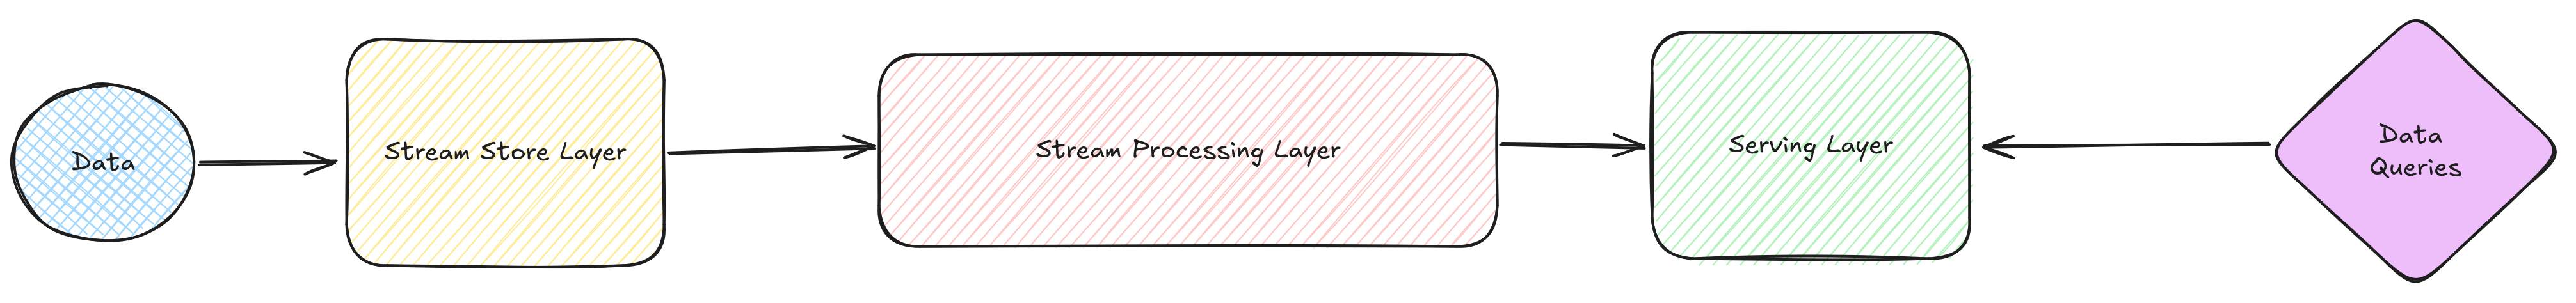
\includegraphics[width=0.8\textwidth]{teorico/kappa.png}
\caption{Diagrama de la Arquitectura Kappa}
\label{fig:arquitectura_kappa}
\end{figure}

\subsection{Capacidades}
La Arquitectura Kappa ofrece varias capacidades clave:
\begin{itemize}
    \item Reduce la complejidad del sistema al unificar el procesamiento batch y streaming
    \item Mejora la mantenibilidad al no tener que duplicar lógica para los distintos esquemas de procesamiento
    \item Garantiza la coherencia entre los resultados del streaming y el reprocesamiento.
\end{itemize}

\newpage
\subsection{Desafíos}
A pesar de sus ventajas, la Arquitectura Kappa presenta algunos desafíos:
\begin{itemize}
    \item Requiere un incremento en el uso de recursos muy grande cuando es necesario reprocesar los datos históricos.
    \item El costo de retención de eventos a largo plazo son enormes y vuelven prohibitiva esta arquitectura sin cambios.
    \item Es necesario reprocesar toda la historia en caso de que exista la necesidad de borrado de información
\end{itemize}


% \subsection{Conclusiones}
% La Arquitectura Kappa representa una alternativa interesante en el diseño de sistemas de procesamiento de datos, 
% ofreciendo una solución elegante para unificar el procesamiento batch y en tiempo real. 
% Su enfoque en el procesamiento de streams como paradigma único simplifica la arquitectura general y reduce la complejidad del mantenimiento del código.
% \newpage